\documentclass[11pt]{article}
\thispagestyle{empty}
\hoffset        -.7truein
\voffset        -1.1truein
\oddsidemargin  0mm
\topmargin      0.25truein
\textwidth      7.8truein
\textheight     9.7truein

\usepackage{graphicx}
\usepackage{epsfig}
\usepackage{amsmath}
\usepackage{fancyhdr}
\usepackage{mathptmx}
\usepackage{mathtools}

\usepackage{amsmath,amsfonts,amsthm,amssymb,graphicx,calc,mathtools,enumitem,array}

\usepackage{tikz}
\usetikzlibrary{calc}
\tikzset{point/.style={circle,inner sep=0pt,minimum size=3pt,fill=black}}
\tikzset{hole/.style={circle,draw=black,inner sep=0pt,minimum size=5pt,fill=white}}
\newcommand*{\TickSize}{2pt}

\newcolumntype{M}[1]{>{\centering\arraybackslash}m{#1}}
\newcolumntype{N}{@{}m{0pt}@{}}
\pagestyle{fancy}
\renewcommand{\headrulewidth}{ 0pt}
\lhead{\tiny\copyright Arpan Pal}


\begin{document}
\Huge
\begin{center}
\textbf{
        Spring 2020 \\
        Math 142 \\
        Exam 1\\
        Form B
}
\end{center}
\Large
\vspace{.65truein}
\begin{quote}
Last Name:\underline{~~~~~~~~~~~~~~~~~~~~~~~~~~~~~~~~~~~~~~~~~~~~~~~~~~~~~}\hspace{.2truein}First
Name:\underline{~~~~~~~~~~~~~~~~~~~~~~~~~~~~~~~~~~~~~~~~~~~~~~~~~~~~~~~}

\vspace{.5truein}
%Exam Seat \#:\underline{~~~~~~~~~~}\hspace{.2truein}
UIN:\underline{~~~~~~~~~~~~~~~~~~~~~~~~~~~~~~~~~~~~~~~~~~~}\hspace{.2truein}Section \#:\underline{~~~~~~~~~~~~~~~}\hspace{.2truein}
%Regular Class Seat \#:\underline{~~~~~~~~~~~}
\end{quote}

\vfill
\begin{quote}
{\bf \Large On my honor, as an Aggie, I have neither given nor received unauthorized aid on
this academic work.}
\end{quote}

\begin{quote}
{\bf \Large Signature:\underline{~~~~~~~~~~~~~~~~~~~~~~~~~~~~~~~~~~~~~~~~~~~~~~~~~~~~~~~~~~~~~~~~~~~~~~~~~~}}
\end{quote}

\normalsize
\vfill
\underline{\bf INSTRUCTIONS}
\begin{itemize}
\item TURN OFF AND PUT AWAY ALL CELL PHONES AND ELECTRONIC DEVICES.  IF AN ELECTRONIC DEVICE (OTHER THAN YOUR CALCULATOR) IS SEEN OR HEARD DURING THE EXAM YOU WILL RECEIVE A ZERO.

\item The gray or blue Texas A\&M University Scantron is required for this exam.

\item Fill in your scantron with the appropriate information.  To avoid a possible $10$ point penalty, you must fill in and bubble your Last Name, First Name, MI, DEPT
(MATH), Course No. (142), Section (505), UIN, and Test Form(A or B).  Please also write ``Arpan" in the Instructor field, ``Exam 1" in the Exam Field, and then sign in the appropriate place.

\item You will have 50 minutes to complete this exam.  As soon as time is called, you must stop writing, put down your pencil, and close your exam.

\item {\bf Part 1: Multiple Choice (Problems 1-10)} Each problem is worth 6 points.  You \textbf{MUST} record your answer on your scantron.  It is highly recommended that you record your answer on your exam as well.  Unless noted otherwise, answer choices are rounded to four decimal places.

\item {\bf Part 2:  Workout (Problem 11-14)}  You are required to show your work on these problems.  An answer with no work is unacceptable.  Please clearly box your final answer.  Each workout problem is worth 10 points.

\end{itemize}
\vfill
\begin{center}
{\bf \LARGE ``An Aggie does not lie, cheat or steal or tolerate those who do."}
\end{center}
\newpage



\begin{quote}
\textbf{Part 1:  Multiple-Choice Problems.}  Each multiple choice question is worth 6 points.  You \textbf{MUST} record your answer on your scantron.  It is highly recommended that you
record your answer on your exam as well.  Unless noted otherwise, answer choices are rounded to four decimal places.
\end{quote}


\begin{enumerate}

\item Use the graph of $f(x)$ below to estimate $\displaystyle\lim_{x\to -3} f(x)$.

\begin{minipage}{2.5truein}
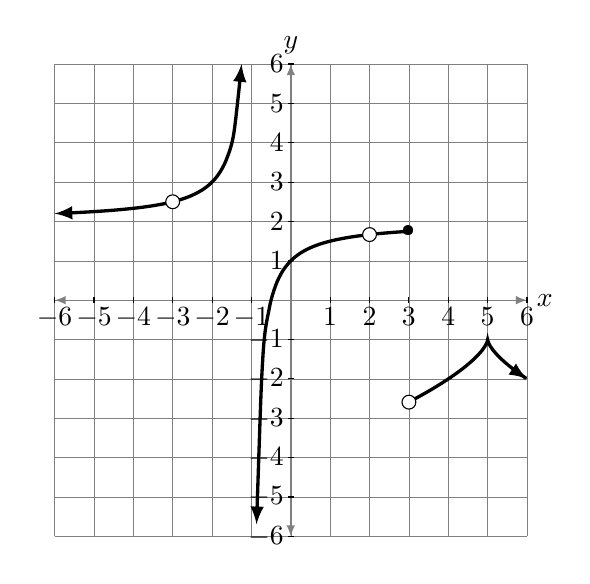
\begin{tikzpicture}[scale=0.5]
\draw [latex-latex, thin, draw=gray] (-6,0) -- (6,0) node [right] {$x$};% x-axis
\draw [latex-latex, thin, draw=gray] (0,-6) -- (0,6) node [above] {$y$};% y-axis
\draw[step=1cm,gray,very thin] (-6,-6) grid (6,6);

\foreach \x in {-6,-5,-4,-3,-2,-1,1,2,3,4,5,6} {%
    \draw ($(\x,0) + (0,-\TickSize)$) -- ($(\x,0) + (0,\TickSize)$)
        node [below] {$\x$};
}

\foreach \y in {-6,-5,-4,-3,-2,-1,1,2,3,4,5,6} {%
    \draw ($(0,\y) + (-\TickSize,0)$) -- ($(0,\y) + (\TickSize,0)$)
        node [left] {$\y$};
}
\draw[latex-latex,very thick,domain=-6:-1.25,smooth,variable=\x] plot ({\x},{(2*\x+1)/(\x+1)});
\draw[latex-,very thick,domain=-0.87:3,smooth,variable=\x] plot ({\x},{(2*\x+1)/(\x+1)});
\draw[very thick,domain=3:4.5,smooth,variable=\x] plot ({\x},{-(abs(\x-5))^(2/3)-1});
\draw[very thick,domain=4.5:5.5,smooth,samples=125,variable=\x] plot ({\x},{-(abs(\x-5))^(2/3)-1});
\draw[-latex,very thick,domain=5.5:6,smooth,variable=\x] plot ({\x},{-(abs(\x-5))^(2/3)-1});
\node[hole] at (-3,5/2) {};
\node[hole] at (2,5/3) {};
\draw (3,7/4) node {\textbullet};
\node[hole] at (3,-2.59) {};

\end{tikzpicture}
\end{minipage}
\hspace{.1truein}
\begin{minipage}{4truein}
\begin{enumerate}
\item $0\leq \displaystyle\lim_{x\to 2} f(x)\leq 1$.
\item $\displaystyle\lim_{x\to 2} f(x)$ Does Not Exist.
\item $1\leq \displaystyle\lim_{x\to 2} f(x)\leq 2$.
\item $\displaystyle\lim_{x\to 2} f(x)=3$.
\item $\displaystyle\lim_{x\to 2} f(x)=-2.5$.
\end{enumerate}
\end{minipage}

\vfill
\item Find $\displaystyle\lim_{x\to10} \frac{x+10}{x-10}$, if it exists. If it does not exist, use limits to describe the way in which it does not exist. \vskip 2em
\begin{enumerate}
    \item The limit does not exist and $\displaystyle\lim_{x\to10^{-}}f(x) \rightarrow \infty$ and $\displaystyle\lim_{x\to10^{+}}f(x) \rightarrow -\infty$. \vskip .5em
    \item The limit does not exist and  $\displaystyle\lim_{x\to10}f(x) \rightarrow \infty$ \vskip .5em
    \item The limit does not exist and $\displaystyle\lim_{x\to10^{-}}f(x) \rightarrow -\infty$ and $\displaystyle\lim_{x\to10^{+}}f(x) \rightarrow \infty$. \vskip .5em %Answer
    \item The limit exists, and it equals 0. \vskip .5em
    \item The limit exists, and it equals 1.
\end{enumerate}

\vfill

\item Complete the table below for $f(x)=\displaystyle\frac{x-3}{\ln{(x-2)}}$ and then use it to determine which of the following statements below is TRUE. (Answers below are rounded to six decimal places.)

\begin{tabular}{|c|c|c|c|c|c|}
\hline
$x$&2.9&2.99&3&3.01&3.1\\
\hline
$f(x)$&$\phantom{1111111111}$&$\phantom{1111111111}$&$\phantom{1111111111}$&$\phantom{1111111111}$&$\phantom{1111111111}$ \\
\hline
\end{tabular}

\begin{enumerate}
\item $f(3.1)=1.000500$ and based on the table above it appears that $\displaystyle\lim_{x\to 3} f(x)\approx 1$.\vskip .5em
\item $f(3.01)=1.004992$ and based on the table above it appears that $\displaystyle\lim_{x\to 1} f(x)\approx 3$.\vskip .5em
\item $f(2.99)=1.233152$ and based on the table above it appears that $\displaystyle\lim_{x\to 1} f(x)\approx 3$.\vskip .5em
\item $f(2.9)=0.949122$ and based on the table above it appears that $\displaystyle\lim_{x\to 3} f(x)\approx 1$.\vskip .5em
\item None of the above statements are true.
\end{enumerate}


\vfill


\newpage

\item Consider the function $f(x)=
    \begin{cases}
        x^2-2 & x\leq 2  \\
        4-x & x>2 \\
    \end{cases}$. Mark the correct option.
\begin{enumerate}
 
 \item $f(x)$ is continuous but not differentiable at $x=2$.\vskip .5em
 \item $f(x)$ is differentiable at $x=2$.\vskip .5em
 \item $f(x)$ is defined but not continuous at $x=2$.\vskip .5em 
 \item $f(x)$ is not defined at $x=2$.\vskip .5em
 \item None of the above.
\end{enumerate}

\vfill
\item Here is the graph of $f(x)$. Which of the following statements below is TRUE?

\begin{minipage}{2.5truein}
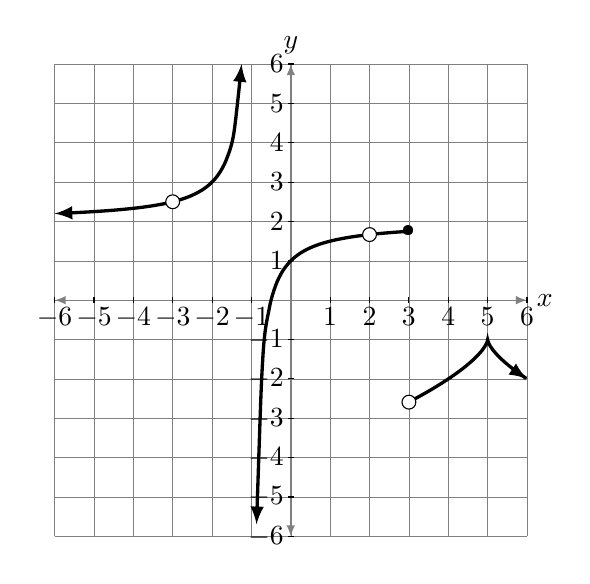
\begin{tikzpicture}[scale=0.5]
\draw [latex-latex, thin, draw=gray] (-6,0) -- (6,0) node [right] {$x$};% x-axis
\draw [latex-latex, thin, draw=gray] (0,-6) -- (0,6) node [above] {$y$};% y-axis
\draw[step=1cm,gray,very thin] (-6,-6) grid (6,6);

\foreach \x in {-6,-5,-4,-3,-2,-1,1,2,3,4,5,6} {%
    \draw ($(\x,0) + (0,-\TickSize)$) -- ($(\x,0) + (0,\TickSize)$)
        node [below] {$\x$};
}

\foreach \y in {-6,-5,-4,-3,-2,-1,1,2,3,4,5,6} {%
    \draw ($(0,\y) + (-\TickSize,0)$) -- ($(0,\y) + (\TickSize,0)$)
        node [left] {$\y$};
}
\draw[latex-latex,very thick,domain=-6:-1.25,smooth,variable=\x] plot ({\x},{(2*\x+1)/(\x+1)});
\draw[latex-,very thick,domain=-0.87:3,smooth,variable=\x] plot ({\x},{(2*\x+1)/(\x+1)});
\draw[very thick,domain=3:4.5,smooth,variable=\x] plot ({\x},{-(abs(\x-5))^(2/3)-1});
\draw[very thick,domain=4.5:5.5,smooth,samples=125,variable=\x] plot ({\x},{-(abs(\x-5))^(2/3)-1});
\draw[-latex,very thick,domain=5.5:6,smooth,variable=\x] plot ({\x},{-(abs(\x-5))^(2/3)-1});
\node[hole] at (-3,5/2) {};
\node[hole] at (2,5/3) {};
\draw (3,7/4) node {\textbullet};
\node[hole] at (3,-2.59) {};

\end{tikzpicture}
\end{minipage}
\hspace{.1truein}
\begin{minipage}{4truein}
\begin{enumerate}

\item The graph of $f(x)$ is continuous at $x=3$.\vskip .5em
\item The graph of $f(x)$ is continuous at $x=5$.\vskip .5em
\item The graph of $f(x)$ is continuous at $x=2$.\vskip .5em
\item The graph of $f(x)$ is continuous at $x=-1$.\vskip .5em
\item The graph of $f(x)$ is continuous at $x=-3$.



\end{enumerate}
\end{minipage}
\vfill



\item What is the average rate of change of the function $f(x)=\displaystyle\frac{x^3}{5}$ on the interval $[1,2]$?
\begin{enumerate}
\item $0$ \vskip .5em
\item $0.4$ \vskip .5em
\item $1$ \vskip .5em
\item $1.4$ \vskip .5em
\item None of the above.
\end{enumerate}



%\vfill
%\item (\# 7 - Jessica) Suppose we are given that $f'(16)=20.82$ for a function $f(x).$ Choose the answer choice below that does NOT necessarily reflect a possible interpretation of this information. \vskip 1em
%\begin{enumerate}
%    \item At $x=16$ on the graph of $f(x)$, the function is positive. \vskip .5em %Answer
%    \item Suppose $f(x)$ is the position function. At 16 seconds, an object is moving at a velocity of 20.82 m/s. \vskip .5em
%    \item Suppose $f(x)$ is the total revenue function. The revenue from selling the 17th widget is \$20.82. \vskip .5em
%    \item At $x=16$, the slope of the line tangent to $f(x)$ is 20.82. \vskip .5em
%   \item All of the above are possible interpretations of the given information.
%\end{enumerate}


\vfill
\newpage

\item Given the graph of $f(x)$ below, for what value(s) of $x$ is $f(x)$ differentiable?

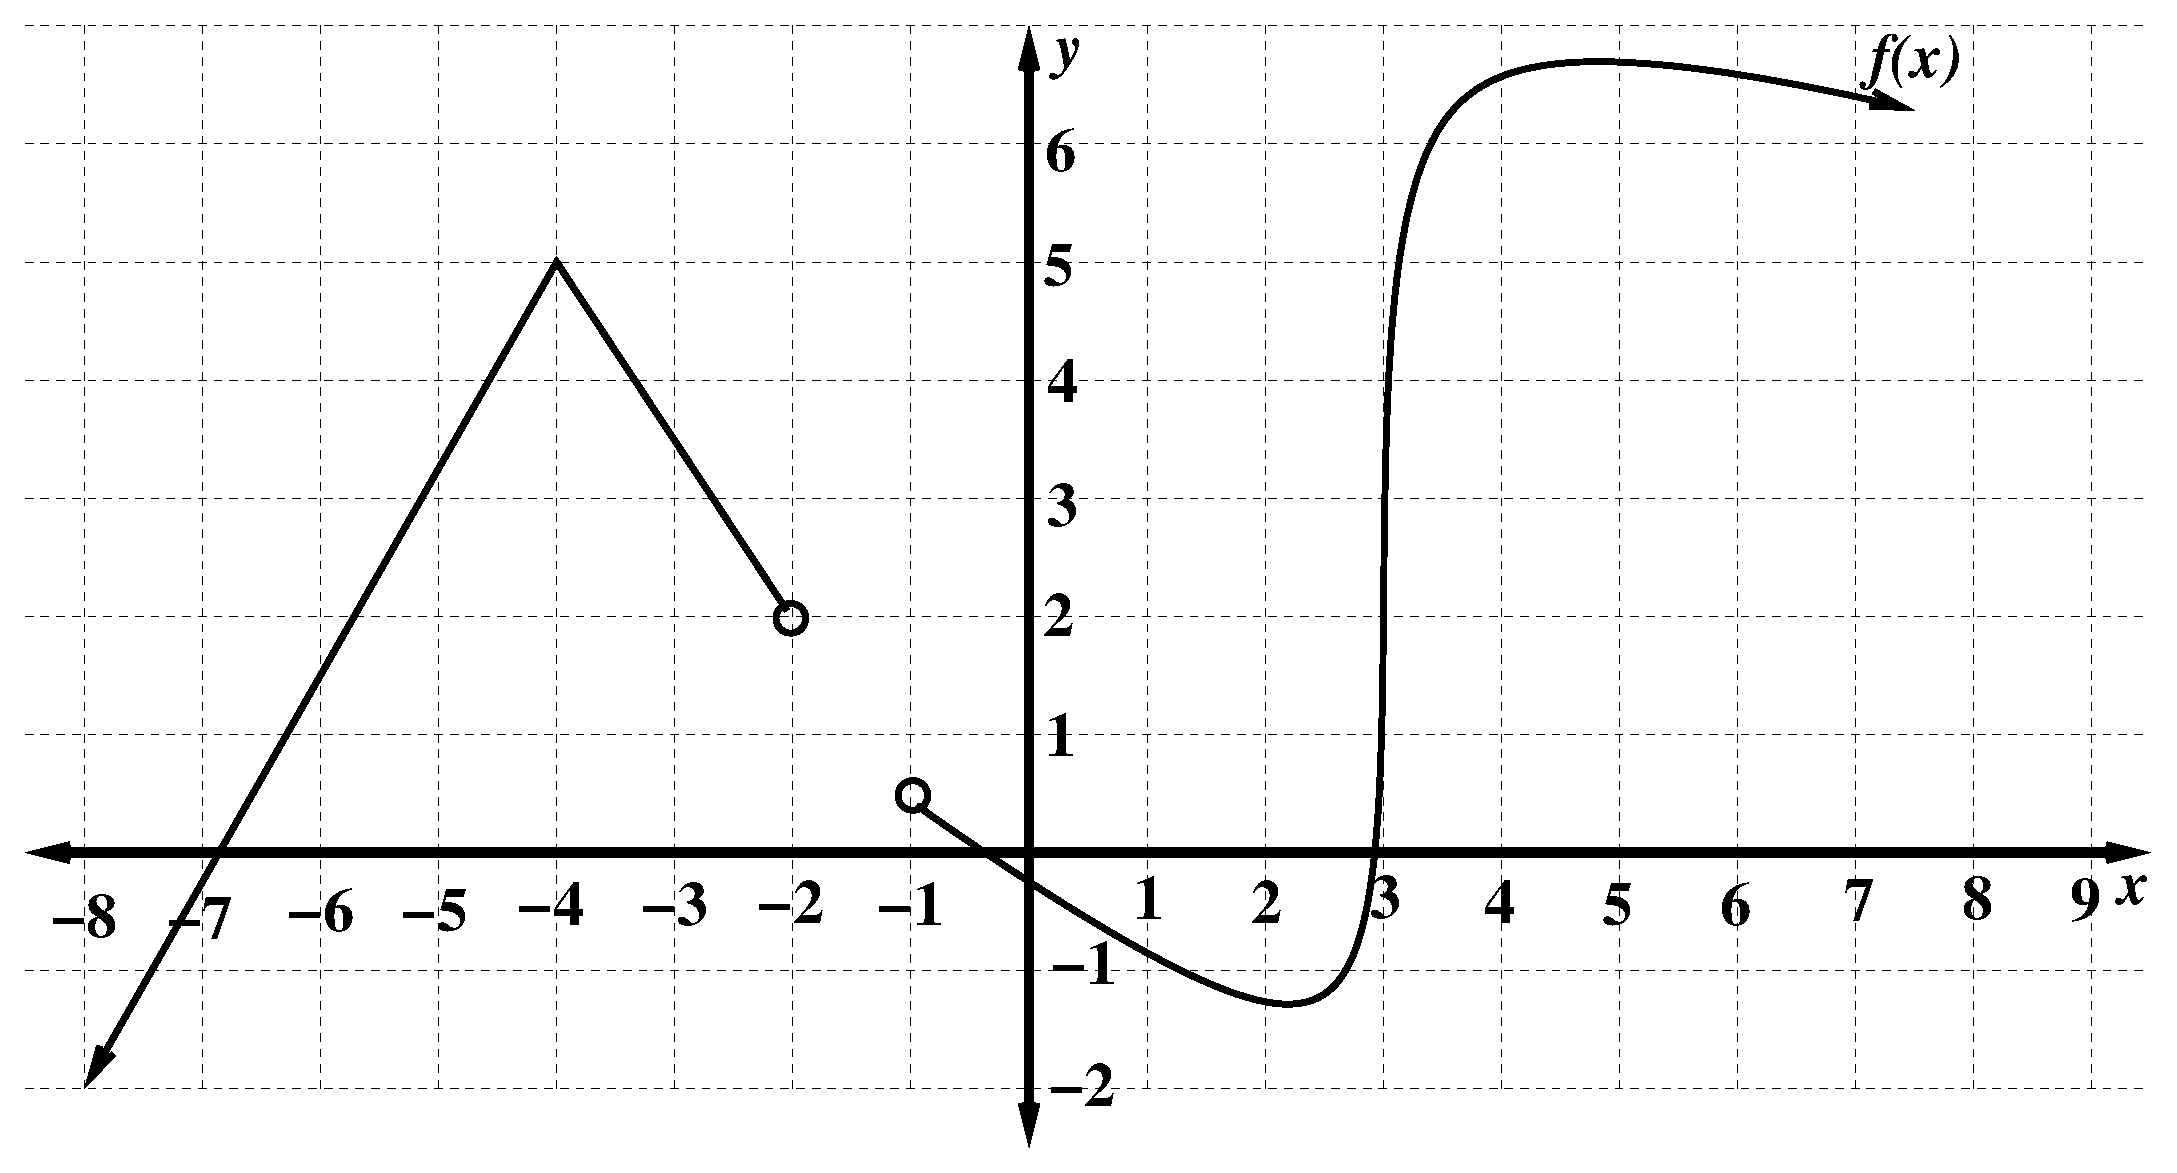
\epsfig{file=14215ax1fig1.eps, width=3truein}

\begin{enumerate}
\item $(-\infty,-4)\cup (-4,-2)\cup (-1,3)\cup (3,\infty)$
\item $(-\infty,-4)\cup (-4,-2)\cup (-2,\infty)$
\item $(-\infty,-4)\cup (-4,-2)\cup (-1,\infty)$
\item $(-\infty,-2)\cup (-1,\infty)$


\item None of the above
\end{enumerate}


\vfill

\item Let $C(x)=x^{3/2}+12x^{1/2}+50$ be the cost in dollars for Sbisa Dining Hall to serve $x$ people lunch in a day. Find the marginal cost function and use it to estimate the cost of the 26th lunch they make in a day.
\begin{enumerate}
\item $\$10.0$\vskip .5em
\item $\$9.7$\vskip .5em
\item $\$8.7$\vskip .5em
\item $\$8.5$\vskip .5em
\item $\$8.0$
\end{enumerate}

\vfill
\item If $\displaystyle{k(x)=3e^{x}-\sqrt{x^5}+\ln\left(\frac{2}{x^4}\right)-8}$, find its derivative. \vskip 1em
\begin{enumerate}
    
    \item $\displaystyle{k'(x)=3e^x+\frac{5}{2}\sqrt{x^3}-3x}$ \vskip .5em
    \item $\displaystyle{k'(x)=3e^x-\frac{5}{2}\sqrt{x^3}-\frac{4}{x}-2^3}$ \vskip .5em
    \item $\displaystyle{k'(x)=3e^x-\frac{5}{2}\sqrt{x^3}-\frac{4}{x}}$ \vskip .5em%Answer
    \item $\displaystyle{k'(x)=3e^x+\frac{5}{2}\sqrt{x^3}-3x-8}$ \vskip .5em    
    \item None of the above. 
\end{enumerate}
\vfill
\newpage
\item Find the equation of the tangent line to the curve $f(x)=3x^2-4x+7e^x$ at $x=0$.
\begin{enumerate}
    \item $y=3x+11$ \vskip 1em %Answer
    \item $y=-3x+7$ \vskip 1em
    \item $y=-3x+4$ \vskip 1em
    \item $y=3x+7$ \vskip 1em
    \item None of the above
\end{enumerate}

\vfill


\newpage
\begin{center}
{\Huge STOP!!  All of your answers up until this point need to be recorded on your scantron!}

{\small It is highly recommend that you record your answer on your exam as well but the answers marked on the scantron will take precedence if there is a discrepancy.
Please note that the total number of points you received credit for on the scantron portion of the exam will be posted on eCampus but not written on this exam when it is returned to you.}
\end{center}

\textbf{Part 2:  Workout Problems.}  You are required to show your work on these problems.  An answer with no work is unacceptable.  Please clearly box your final answer. Each problem is worth 10 points.
\item Consider the function $f(x)=\displaystyle\frac{x^3e^x}{x^2-3}$.  Find $f'(x)$ (Do not simplify).
\vfill
\item Given the graph of $f(x)$ below, sketch a graph of $f'(x)$.  Clearly label at least two points on the graph of $f'(x)$.

\begin{minipage}{3truein}
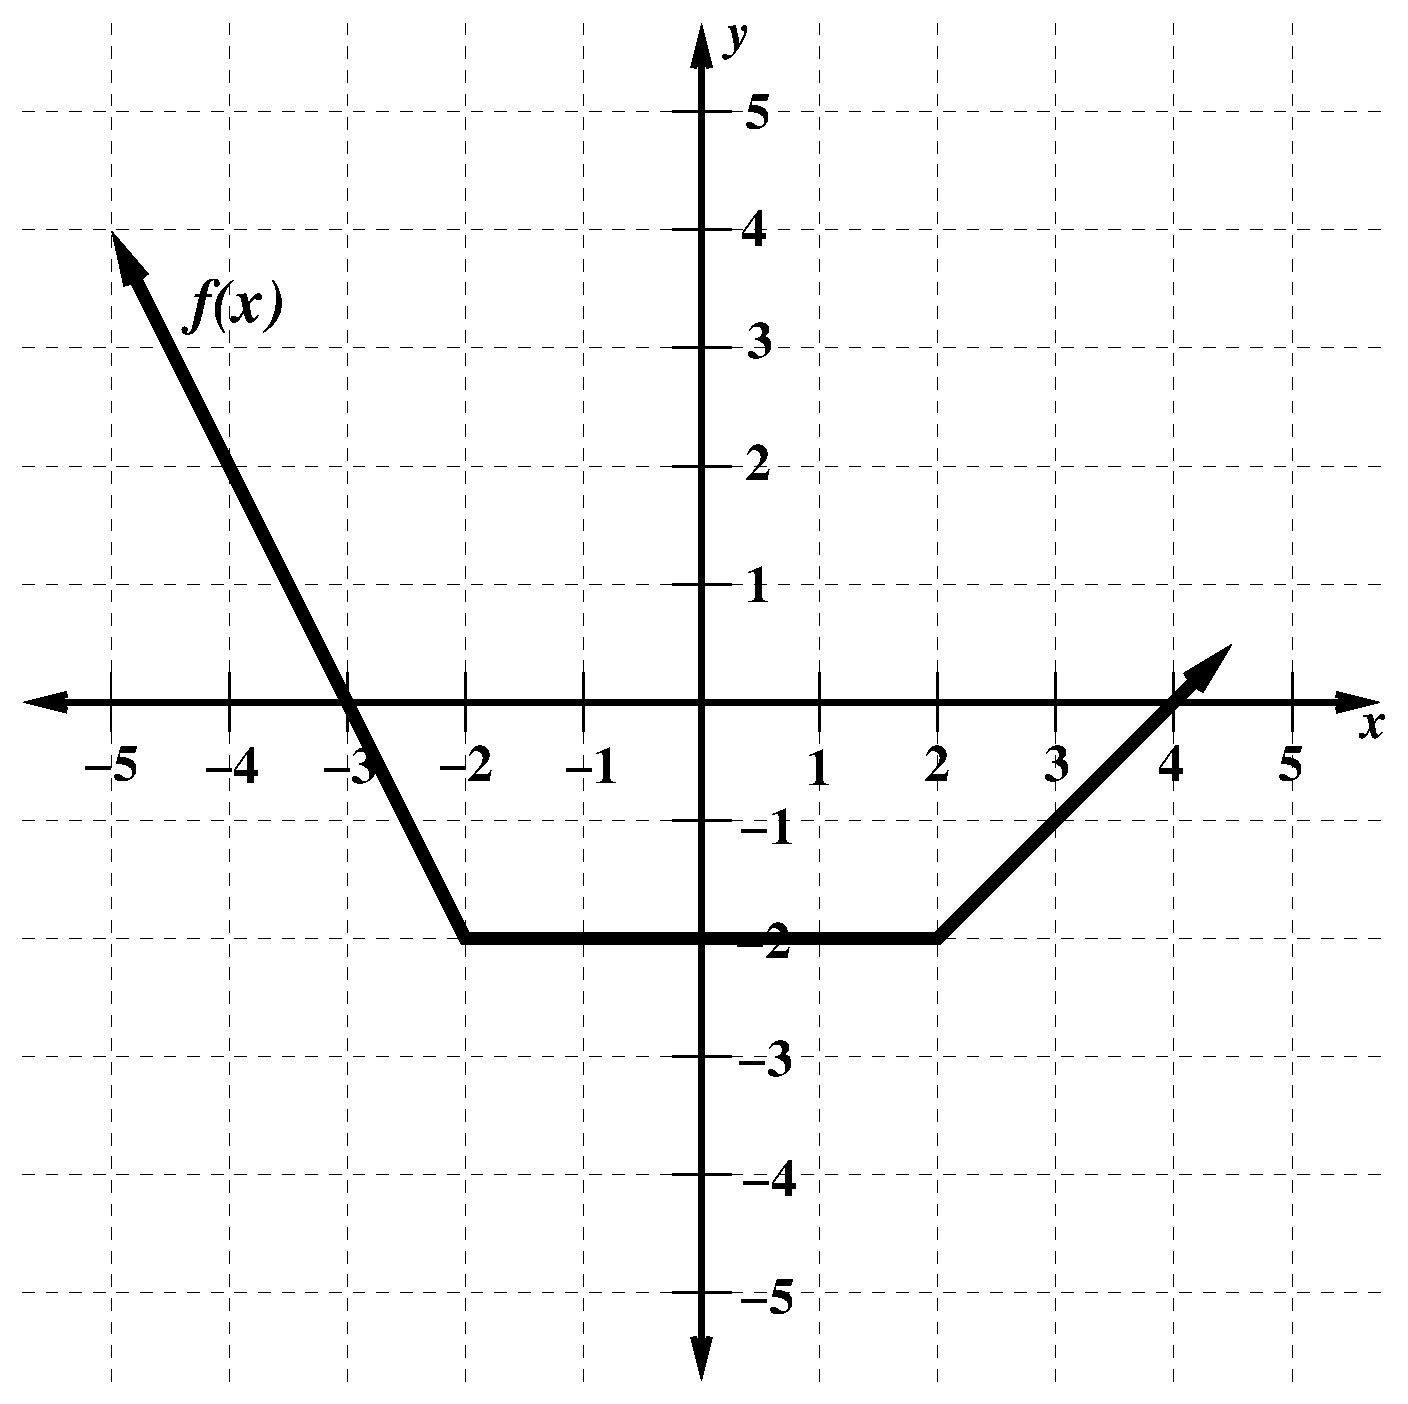
\epsfig{file=14220ax1fig1.eps, width=3truein}
\end{minipage}
\hspace{.3truein}
\begin{minipage}{3truein}
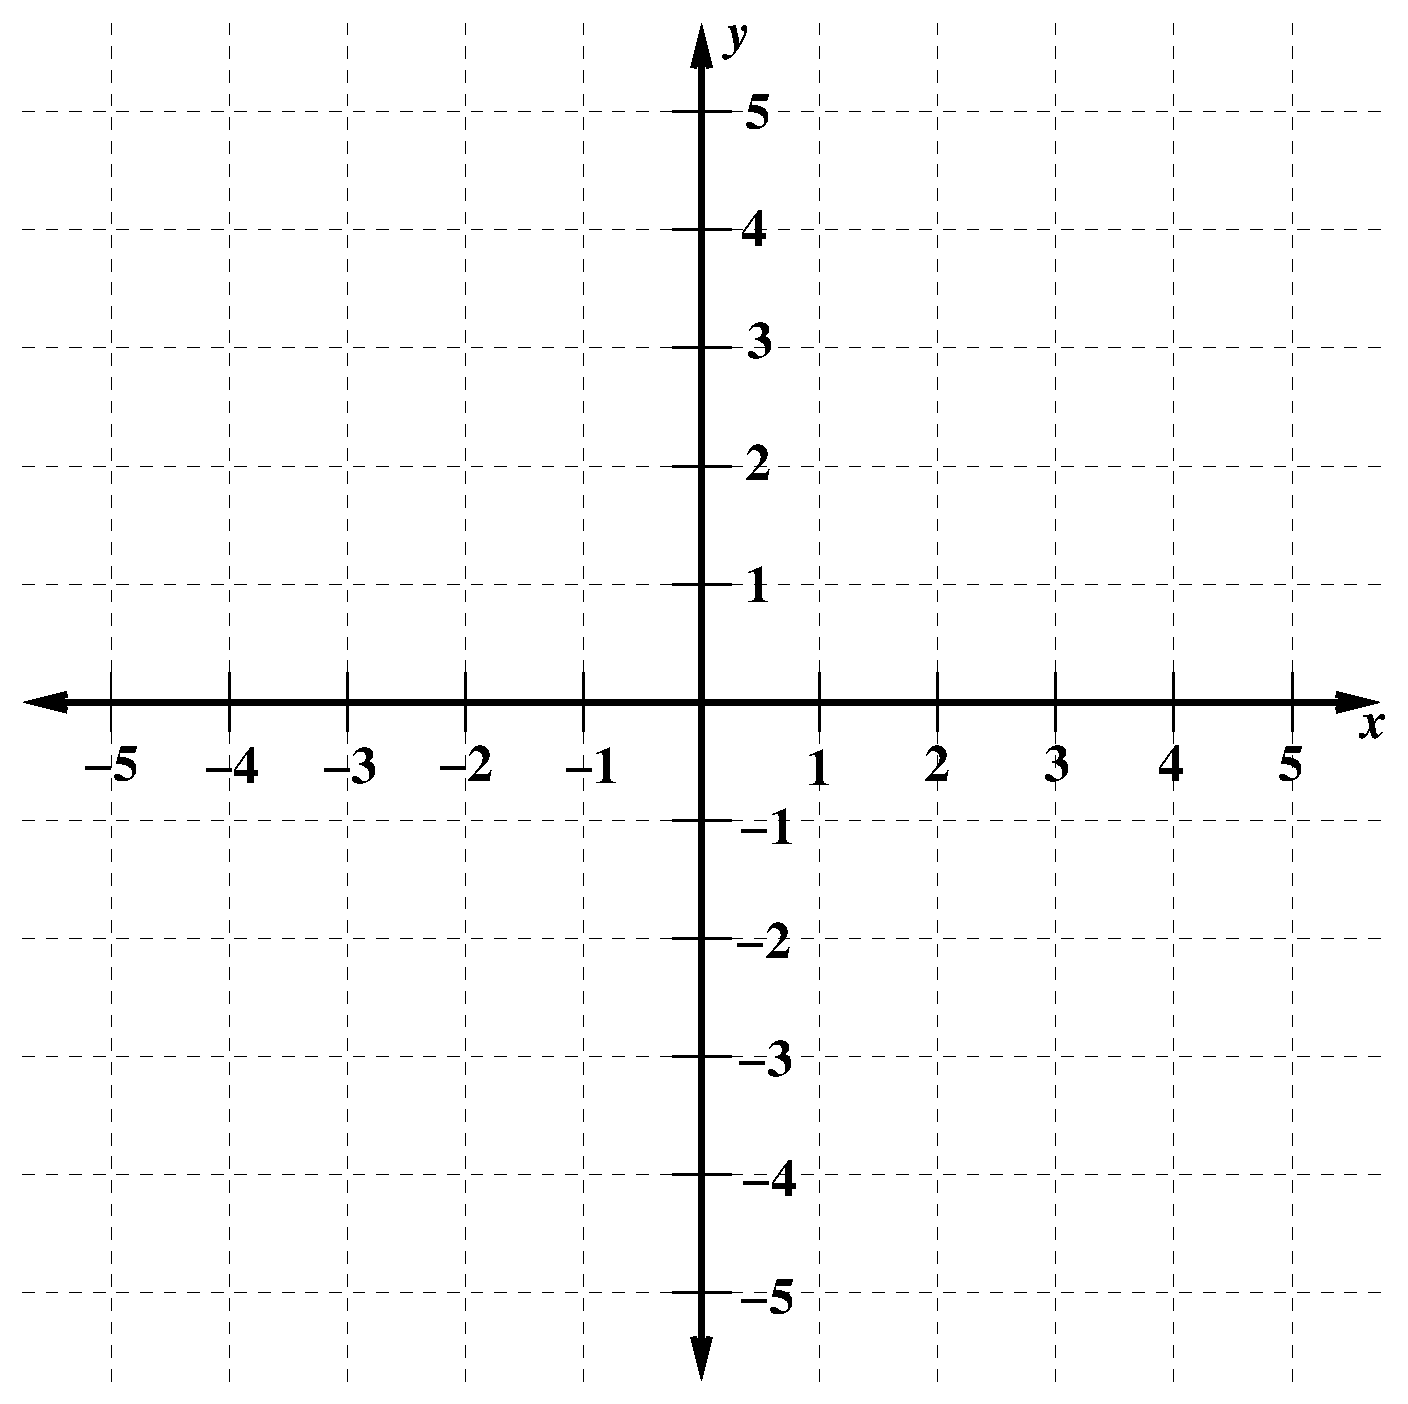
\epsfig{file=14220ax1fig2.eps, width=3truein}
\end{minipage}

\vfill

\newpage
\item Consider the function $f(x)=3x^2+5x-9$.  Use the limit definition of the derivative to find $f'(x)$.

\vfill

\item Algebraically evaluate the limit below.  You must show all of your work like we did in-class.

$\displaystyle\lim_{x\to 5} \displaystyle\frac{x^2-2x-15}{x^2-7x+10}$


\vfill
\hspace{.25truein}The total number of points you received credit for on the workout portion of the exam is \hspace{.1truein} 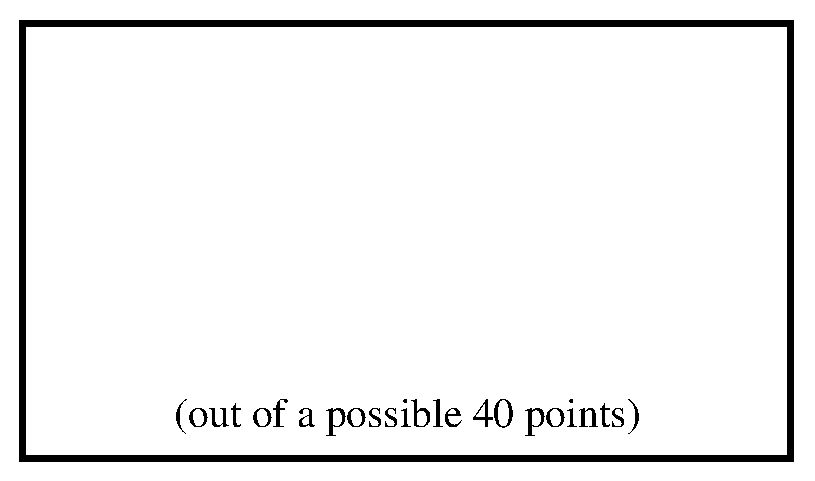
\epsfig{file=14019cxbox.eps, width=1.5truein}.

\vspace{.1truein}
\hspace{.25truein}  Please fill in these blank: \hspace{.05truein} Name:\underline{~~~~~~~~~~~~~~~~~~~~~~~~~~~~~~~~~~~~~~~~~~~~~~~~~~~~~~~~~~~~~~~~~~~~~~~~~~~~~~~~~~~~~~~~~~~~~~~~~~~~~~~~~~~~~~~~~~~~~~~~~~~~~~~~~~~}.

%\newpage
%\begin{center}
%In case you finish early, here is a puzzle for you to work on.

%I would highly recommend that you look over your work instead of doing this puzzle!
%\end{center}

%\begin{figure}[ht!]
%\centering
%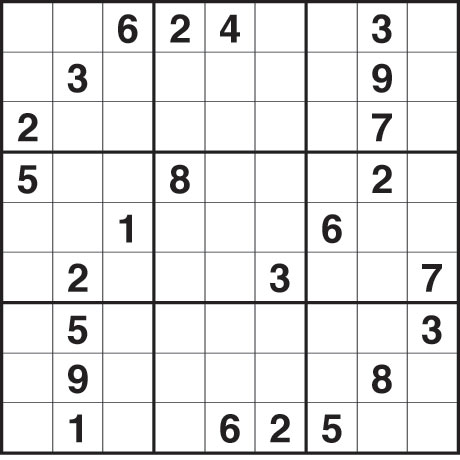
\includegraphics[width=60mm]{medium-sudoku-1.jpg}
%\end{figure}




\end{enumerate}
\end{document}
